% -*- mode: latex; mode: flyspell; ispell-local-dictionary: "en_US"; coding: utf-8; fill-column: 80 -*-

\documentclass{article}

\usepackage[utf8]{inputenc}
\usepackage[english]{babel}

\usepackage{amsmath,amsfonts,amssymb}
\usepackage{fullpage}
\usepackage{verbatim}

\usepackage{tikz,pgfplots}
\usetikzlibrary{patterns, patterns.meta}

\pgfplotsset{
  width = 150mm,
  height = 100mm,
  major grid style = { thin, dotted, color = black!50 },
  minor grid style = { thin, dotted, color = black!50 },
  grid,
  xtick distance = 1,
  ymin = 0,
  every axis/.append style = {
    line width = 0.5pt,
    tick style = {
      line cap = round,
      thin,
      major tick length = 4pt,
      minor tick length = 2pt,
    },
  },
  legend cell align = left,
  legend pos = north west,
  enlarge x limits = 0.25,
	/pgfplots/ybar legend/.style = {
		/pgfplots/legend image code/.code={%
			\draw[##1,/tikz/.cd,yshift=-0.25em]
			(0cm,0cm) rectangle (3pt,0.8em);},
	},  
}

% Extrapolate Kaneta's Numbers
% text     | pc    | pshufb | pext  | rel-pshufb                         | rel-pext                           | got pc
% dblp.xml | 2.99  | 3.09   | 3.04  | 1,033444816053511705685618729097   | 1,0167224080267558528428093645485  |
% dna      | 2.42  | 2.07   | 2.05  | 0,85537190082644628099173553719008 | 0,8471074380165289256198347107438  |
% english  | 27.2  | 23.7   | 23.5  | 0,87132352941176470588235294117647 | 0,86397058823529411764705882352941 | 
% pitches  | 0.685 | 0.576  | 0.570 | 0,84087591240875912408759124087591 | 0,83211678832116788321167883211679 |
% proteins | 8.29  | 9.27   | 9.12  | 1,1182147165259348612786489746683  | 1,100120627261761158021712907117   |
% sources  | 2.54  | 2.37   | 2.55  | 0,93307086614173228346456692913386 | 1,0039370078740157480314960629921  |

%%%%%%%%%%%%%%%%%%%%%%%%%%%%%%%%%%%%%%%%%%%%%%%%%%%%%%%%%%%%%%%%%%%%%%%%%%%%%%%%

\begin{document}

\title{WT Benchmark}
\author{Jan-Philipp Tarnowski}
\maketitle


%- IMPORT-DATA stats results-2022-02-06--20-11-52.out
% IMPORT-DATA stats results-2022-02-06--22-26-02.out


\begin{center}
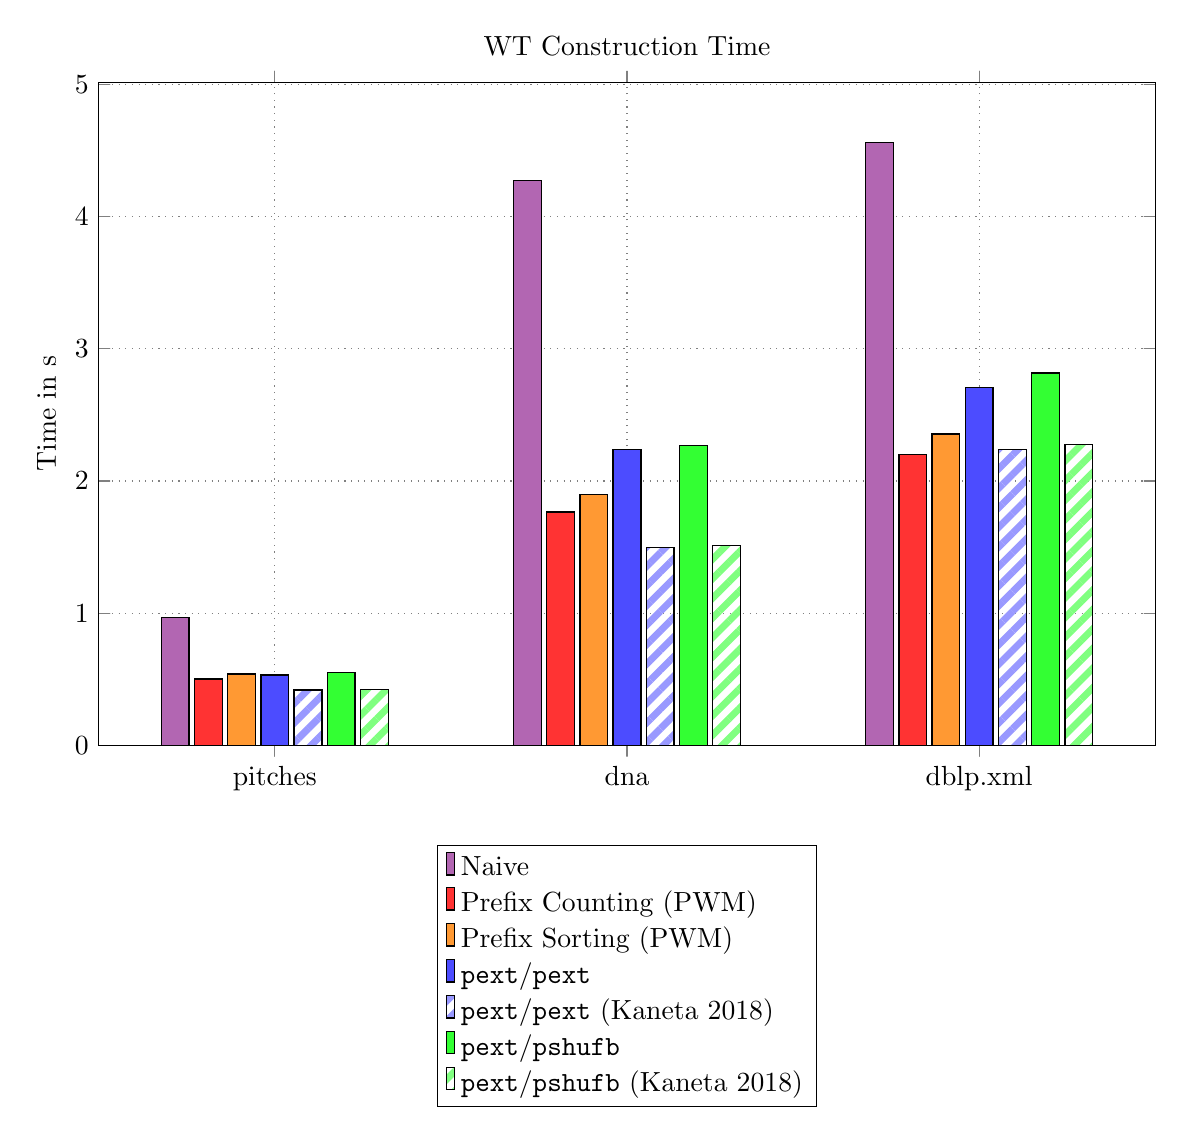
\begin{tikzpicture}
  \begin{axis} [
    ybar,
    xtick = data,
    title = {WT Construction Time},
    legend style = { at = {(0.5, -0.15)}, anchor = north},
	  ylabel = {Time in s},
    symbolic x coords = {
      pitches,   
      dna,
      dblp.xml
    }
  ]



			%%- MULTIPLOT(type) SELECT file AS x, MEDIAN(time_in_s) AS y,MULTIPLOT
			%%- FROM stats WHERE file LIKE '%pitches' OR file LIKE '%dblp.xml' OR file LIKE '%dna' GROUP BY MULTIPLOT,x ORDER BY MULTIPLOT,x
    \addplot[fill = violet!60]                                                                            coordinates { (dblp.xml, 4.56231) (dna, 4.2736)  (pitches, 0.964437) };
    \addplot[fill = red!80]                                                                               coordinates { (dblp.xml, 2.20311) (dna, 1.76648) (pitches, 0.500941) };
    \addplot[fill = orange!80]                                                                            coordinates { (dblp.xml, 2.35551) (dna, 1.89722) (pitches, 0.540171) };
    \addplot[fill = blue!70]                                                                              coordinates { (dblp.xml, 2.70696) (dna, 2.23758) (pitches, 0.530423) };
    \addplot[pattern = {Lines[angle = 45, line width = 2.5pt, distance = 5pt]}, pattern color = blue!40]  coordinates { (dblp.xml, 2.239951304347826) (dna, 1.496398347107438) (pitches, 0.4168414160583941) };
    \addplot[fill = green!80]                                                                             coordinates { (dblp.xml, 2.81672) (dna, 2.26671) (pitches, 0.551705) };
    \addplot[pattern = {Lines[angle = 45, line width = 2.5pt, distance = 5pt]}, pattern color = green!50] coordinates { (dblp.xml, 2.276792608695652) (dna, 1.5109973553719007) (pitches, 0.42122922043795613) };


    \legend{
		  Naive,
      Prefix Counting (PWM),
      Prefix Sorting (PWM),
		  \texttt{pext}/\texttt{pext},
      \texttt{pext}/\texttt{pext} (Kaneta 2018),
      \texttt{pext}/\texttt{pshufb},
      \texttt{pext}/\texttt{pshufb} (Kaneta 2018)
	  };


  \end{axis}
\end{tikzpicture} 
\end{center}

\vspace{1cm}
\begin{tabular}{|lll|}
  \hline
  Text & Size & $\sigma$ \\
  \hline
  pitches & $53.25$ Mib & $132$ \\
  dna & $385.22$ MiB & $16$ \\
  dblp.xml & $282.42$ MiB & $97$ \\
  \hline
\end{tabular}

\pagebreak

\begin{center}
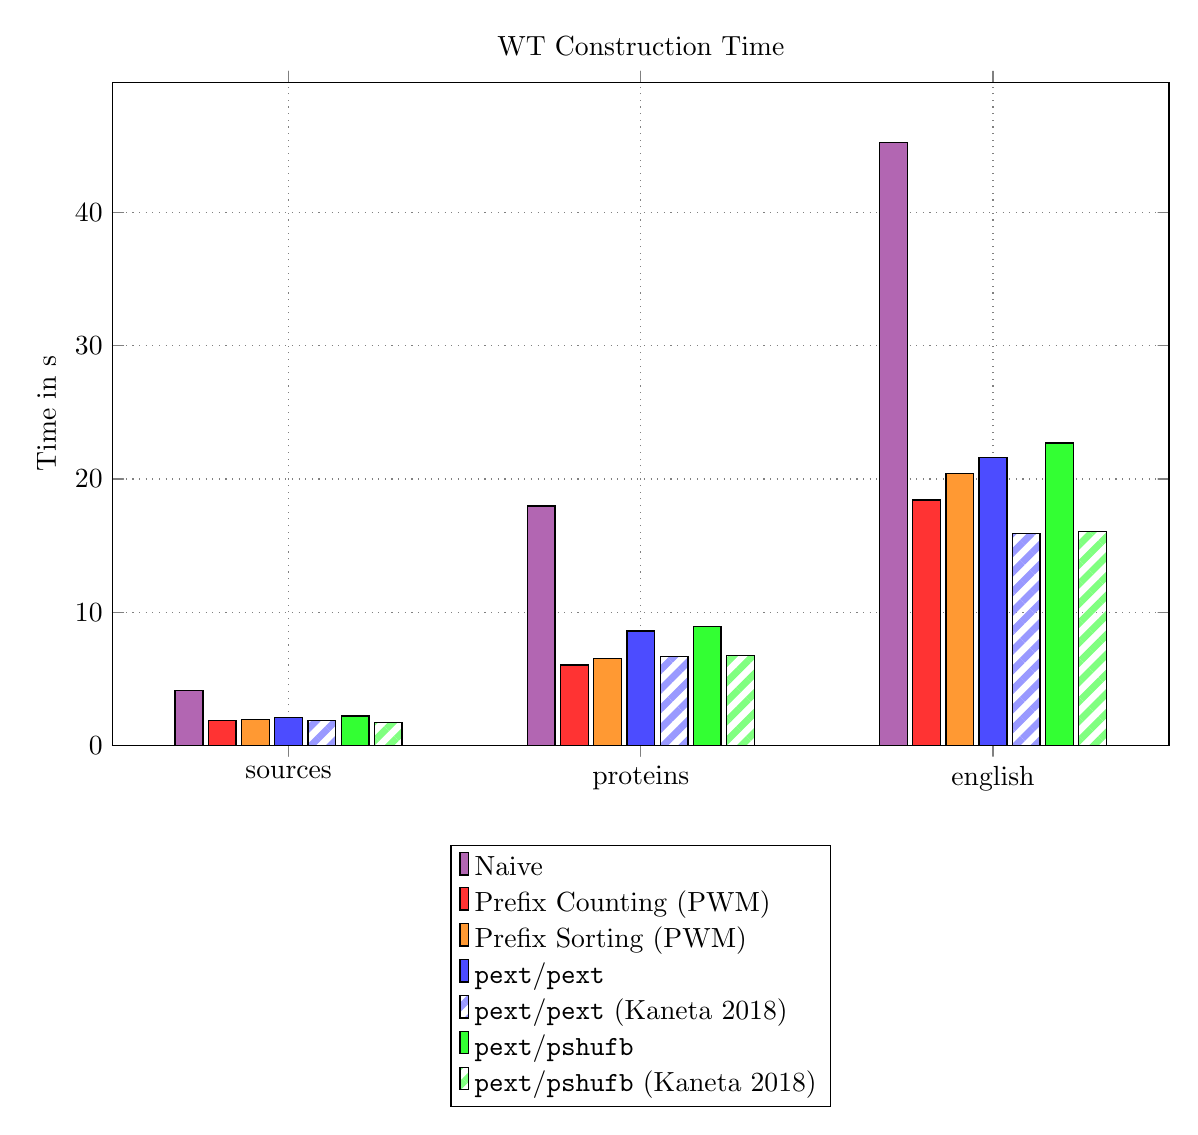
\begin{tikzpicture}
  \begin{axis} [
    ybar,
    xtick = data,
    title = {WT Construction Time},
    legend style = { at = {(0.5, -0.15)}, anchor = north},
	  ylabel = {Time in s},
    symbolic x coords = {
      sources,
      proteins,
      english
    }
  ]


			%%- MULTIPLOT(type) SELECT file AS x, MEDIAN(time_in_s) AS y,MULTIPLOT
			%%- FROM stats WHERE file LIKE '%sources' OR file LIKE '%proteins' OR file LIKE '%english' GROUP BY MULTIPLOT,x ORDER BY MULTIPLOT,x
    \addplot[fill = violet!60]                                                                            coordinates { (english,45.2767) (proteins,17.9848) (sources,4.1178)  };
    \addplot[fill = red!80]                                                                               coordinates { (english,18.431)  (proteins,6.03769) (sources,1.83504) };
    \addplot[fill = orange!80]                                                                            coordinates { (english,20.427)  (proteins,6.50273) (sources,1.9271)  };
    \addplot[fill = blue!70]                                                                              coordinates { (english,21.6085) (proteins,8.57528) (sources,2.10313) };
    \addplot[pattern = {Lines[angle = 45, line width = 2.5pt, distance = 5pt]}, pattern color = blue!40]  coordinates { (english,15.923841911764708) (proteins,6.642187310012062) (sources,1.8422645669291338) };
    \addplot[fill = green!80]                                                                             coordinates { (english,22.7008) (proteins,8.90187) (sources,2.20626) };
    \addplot[pattern = {Lines[angle = 45, line width = 2.5pt, distance = 5pt]}, pattern color = green!50] coordinates { (english,16.059363970588237) (proteins,6.751433811821471) (sources,1.7122223622047243) };


    \legend{
		  Naive,
      Prefix Counting (PWM),
      Prefix Sorting (PWM),
		  \texttt{pext}/\texttt{pext},
      \texttt{pext}/\texttt{pext} (Kaneta 2018),
      \texttt{pext}/\texttt{pshufb},
      \texttt{pext}/\texttt{pshufb} (Kaneta 2018)
	  };

    


  \end{axis}
\end{tikzpicture} 
\end{center}
\vspace{1cm}
\begin{tabular}{|lll|}
  \hline
  Text & Size & $\sigma$ \\
  \hline
  sources & $201.10$ Mib & $229$ \\
  proteins & $1129.20$ MiB & $27$ \\
  english & $2107.98$ MiB & $238$ \\
  \hline
\end{tabular}


%%%%%%%%%%%%%%%%%%%%%%%%%%%%%%%%%%%%%%%%%%%%%%%%%%%%%%%%%%%%%%%%%%%%%%%%%%%%%%%%

\end{document}
